\documentclass[conference]{IEEEtran}
\usepackage{cite}
\usepackage{amsmath}
\usepackage{algorithmic}
\usepackage{array}
\usepackage{url}
\usepackage{graphicx}
\usepackage[portuguese]{babel}
\usepackage[utf8]{inputenc}

\begin{document}

\title{Trabalho Final \\
	de \\
	Teleinformática e Redes 1}

\author{\IEEEauthorblockN{Marcelo de Araujo}
\IEEEauthorblockA{Universidade de Brasilia \\
	Dep. Ciencia da Computacao\\
	15/0016794}
\and
\IEEEauthorblockN{Davi Freitas}
\IEEEauthorblockA{Universidade de Brasilia \\
	Dep. Ciencia da Computacao\\
	15/0033010}
\and
\IEEEauthorblockN{Rafael Chehab}
\IEEEauthorblockA{Universidade de Brasilia \\
	Dep. Ciencia da Computacao\\
	15/0045123}}

\maketitle

\begin{abstract}
The abstract goes here.
\end{abstract}

\IEEEpeerreviewmaketitle

\section{Introdução}
	Simular redes de computadores tem um relevancia enorme para engenheiros, cientistas e projetistas de redes, permite com que uma topologia seja testada previamente antes de, efetivamente,gastar recursos para a implementacao fisica da rede em algum ambiente, poupando dinheiro e tempo.
	
	Neste trabalho temos como objetivo simular uma topologia de rede, com alguns requisitos, para fortalecermos conceitos aprendidos em sala de aula, mais especificamente topicos como camada fisica e de enlace e protocolos utilizados no simulador.
	
	Os requisitos do trabalho sao:
	
	\begin{itemize}
		\item Quatro redes LANs Ethernet (padrao 802.3) 
		\item Duas LANs Wi-Fi sem fio (padrao 802.11x)
		\item Uma rede WAN conectando as outras redes
		\item Minimo de 10 clientes em cada rede
	\end{itemize}

	Assim adotados a topologia indicada pela figura \ref{fig:topologia}.
	
	\begin{figure}[h]
		\centering
		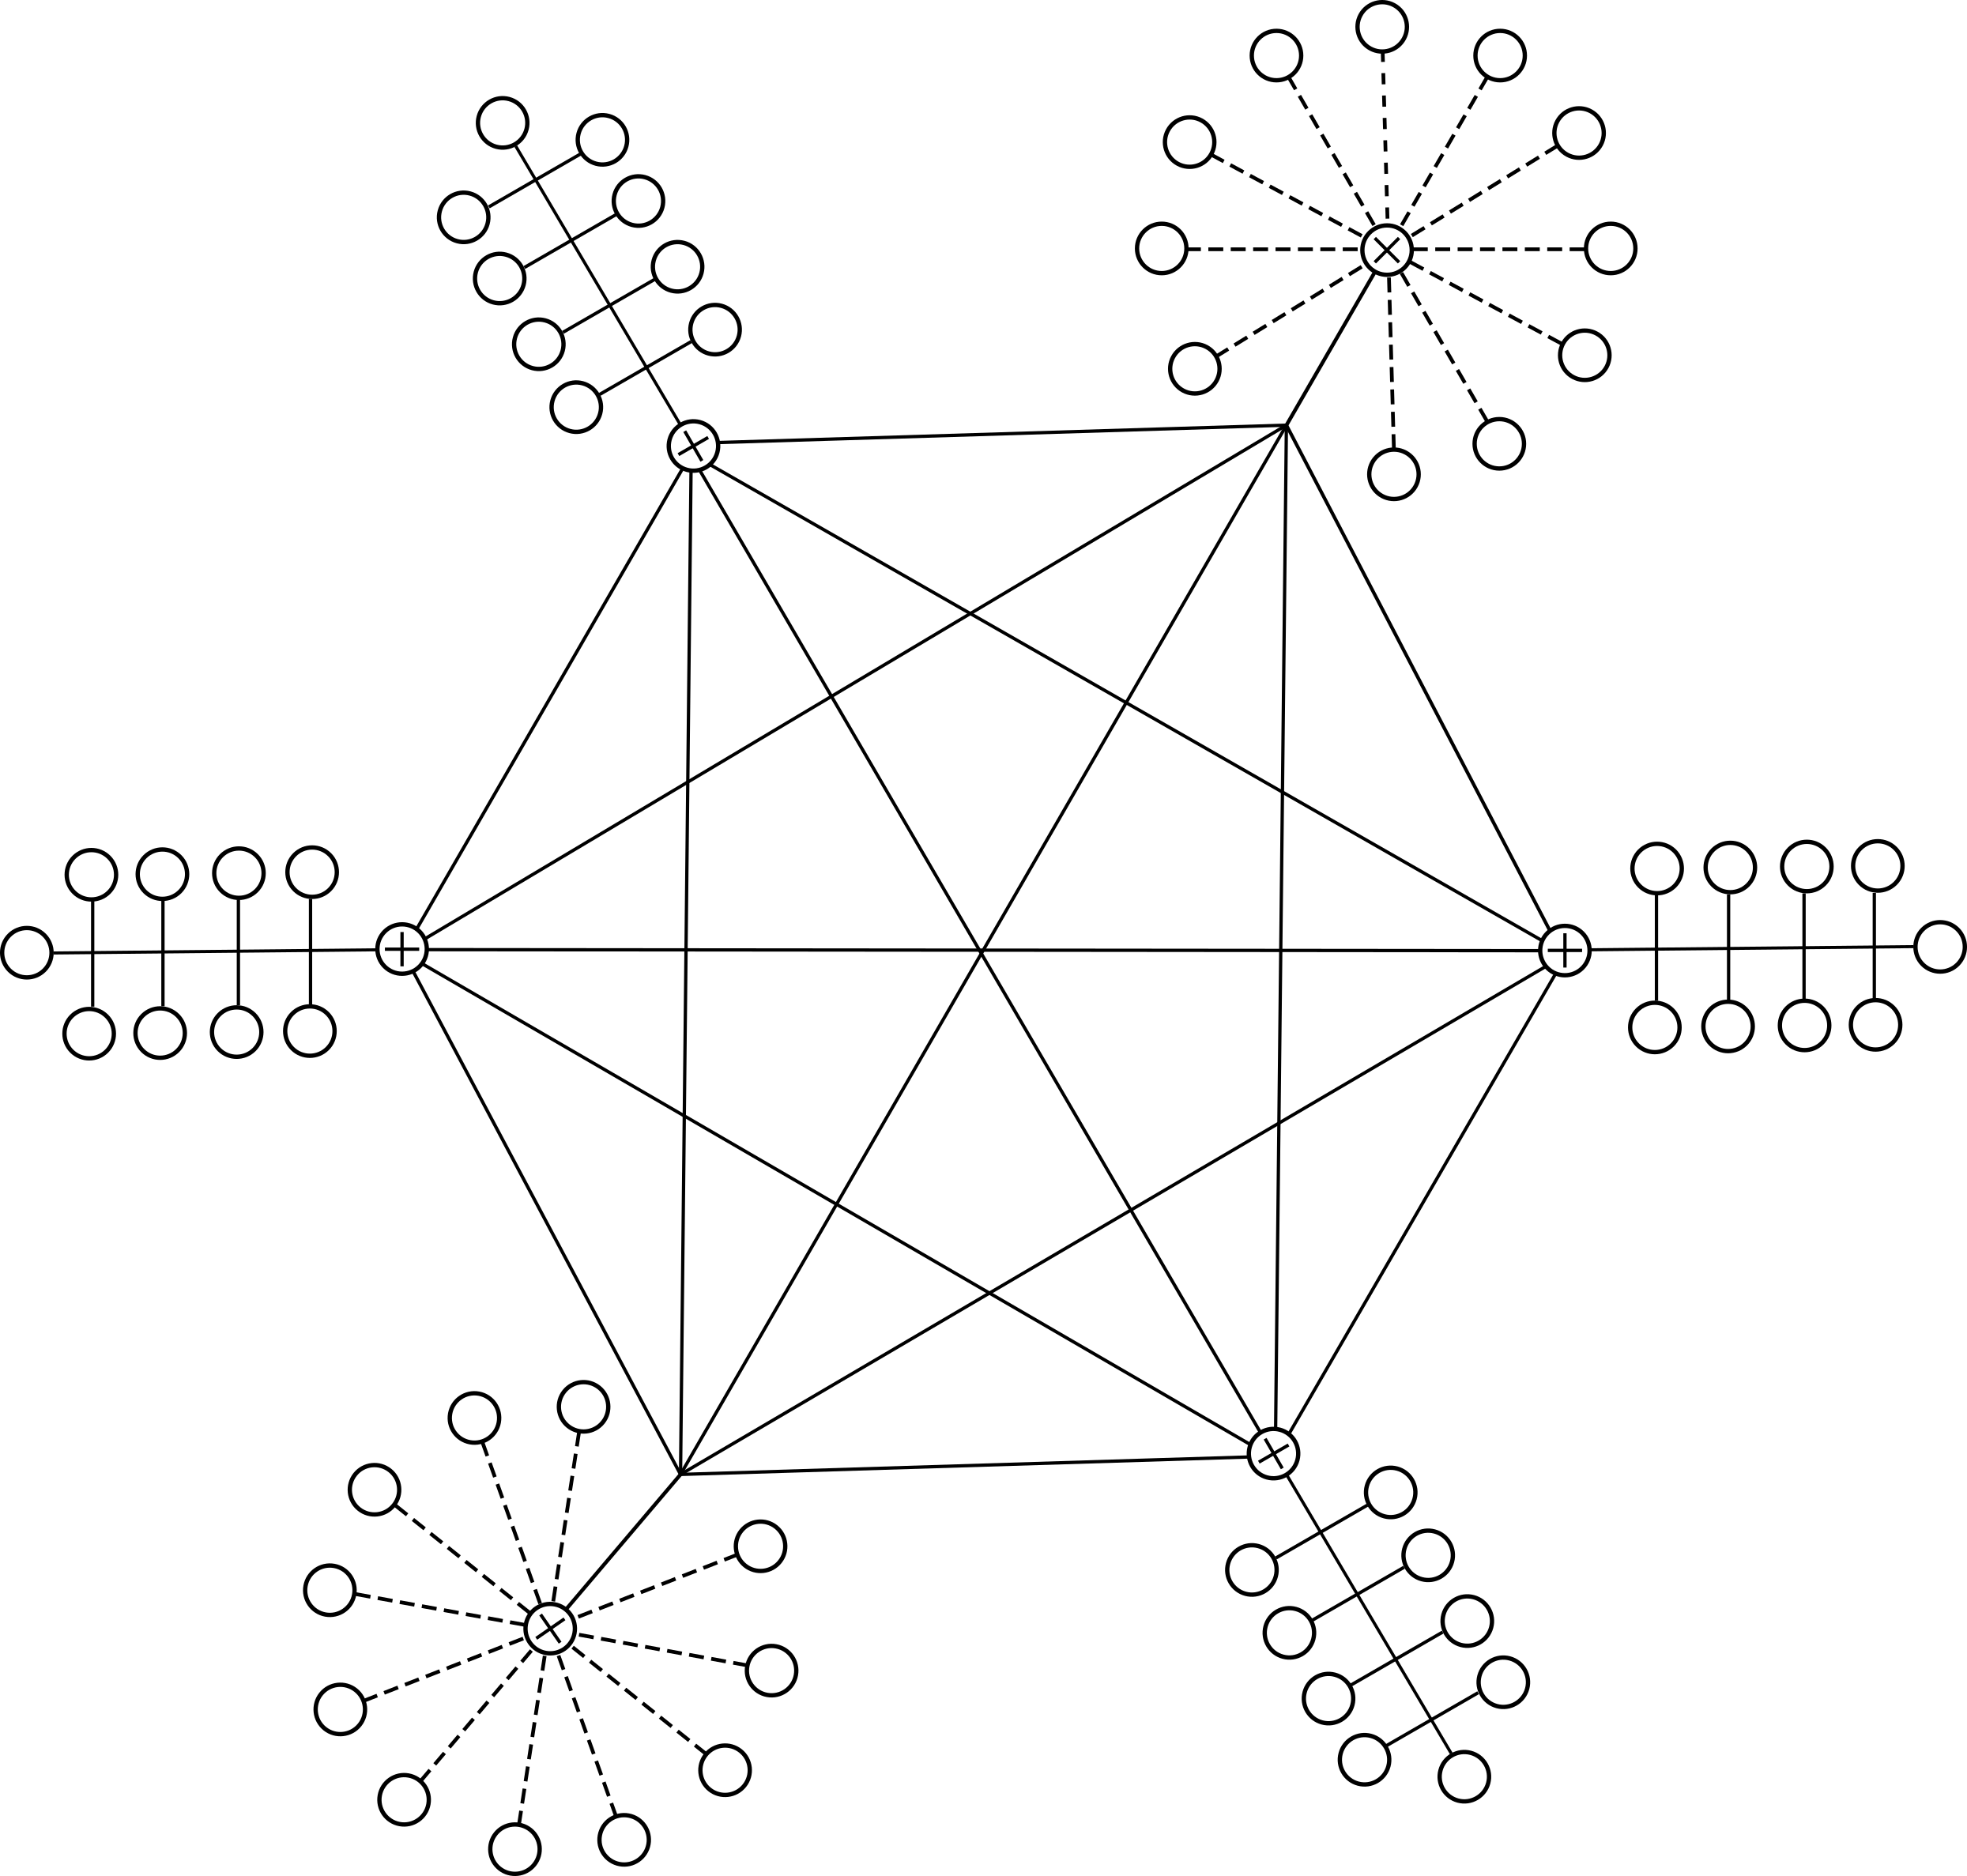
\includegraphics[scale=0.45]{./images/topologia}
		\caption{}
		\label{fig:topologia}
	\end{figure}

\section{Conceitos Teóricos}

\section{Analise Experimental}

\section{Conclusões}



\section*{Agradecimentos}


% that's all folks
\end{document}


